\documentclass[../report.tex]{subfiles}

\graphicspath{{\subfix{../image/}}}

\begin{document}
\subsection{Motordriver PCB}
This is a 2 layer PCB for the Motordriver. 
\begin{figure}[H]
    \centering
    \begin{subfigure}[b]{0.4\linewidth}
      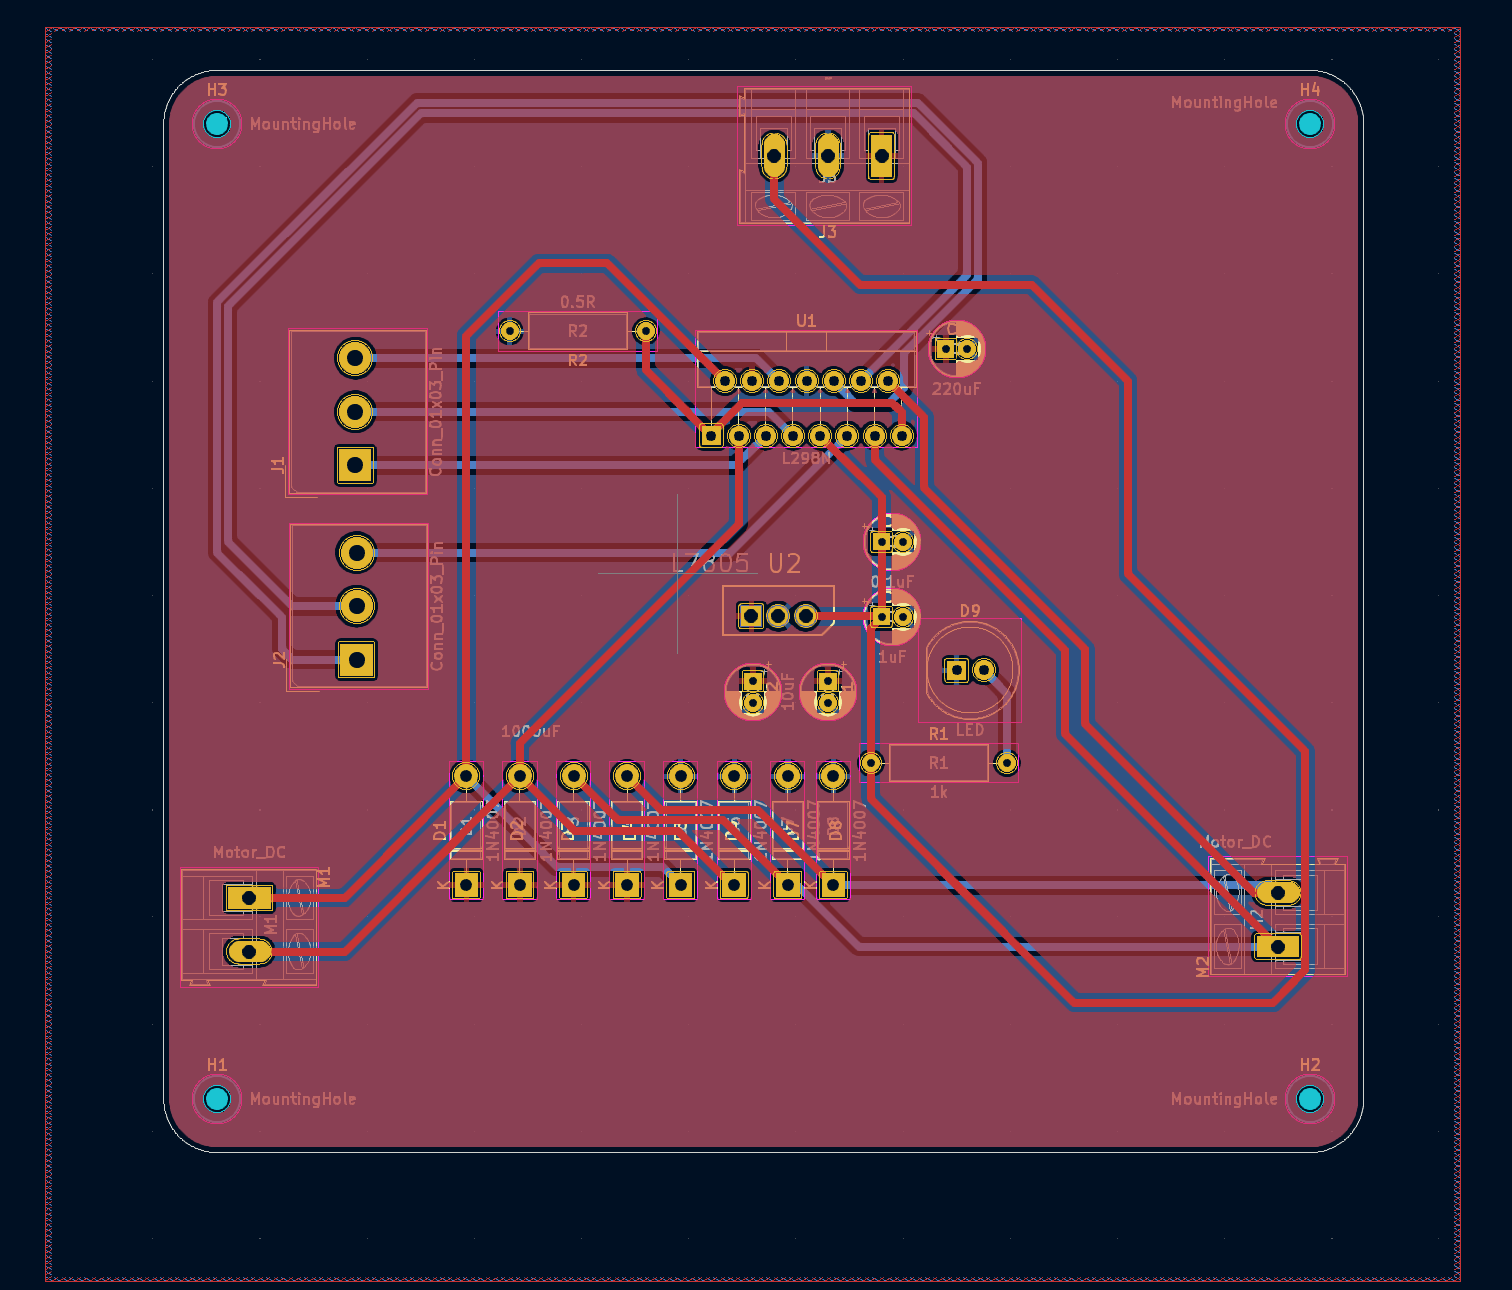
\includegraphics[width=\linewidth]{Screenshot 2023-12-14 at 16.22.46.png}
      \caption{Motordriver PCB} 
    \end{subfigure}
    \begin{subfigure}[b]{0.4\linewidth}
      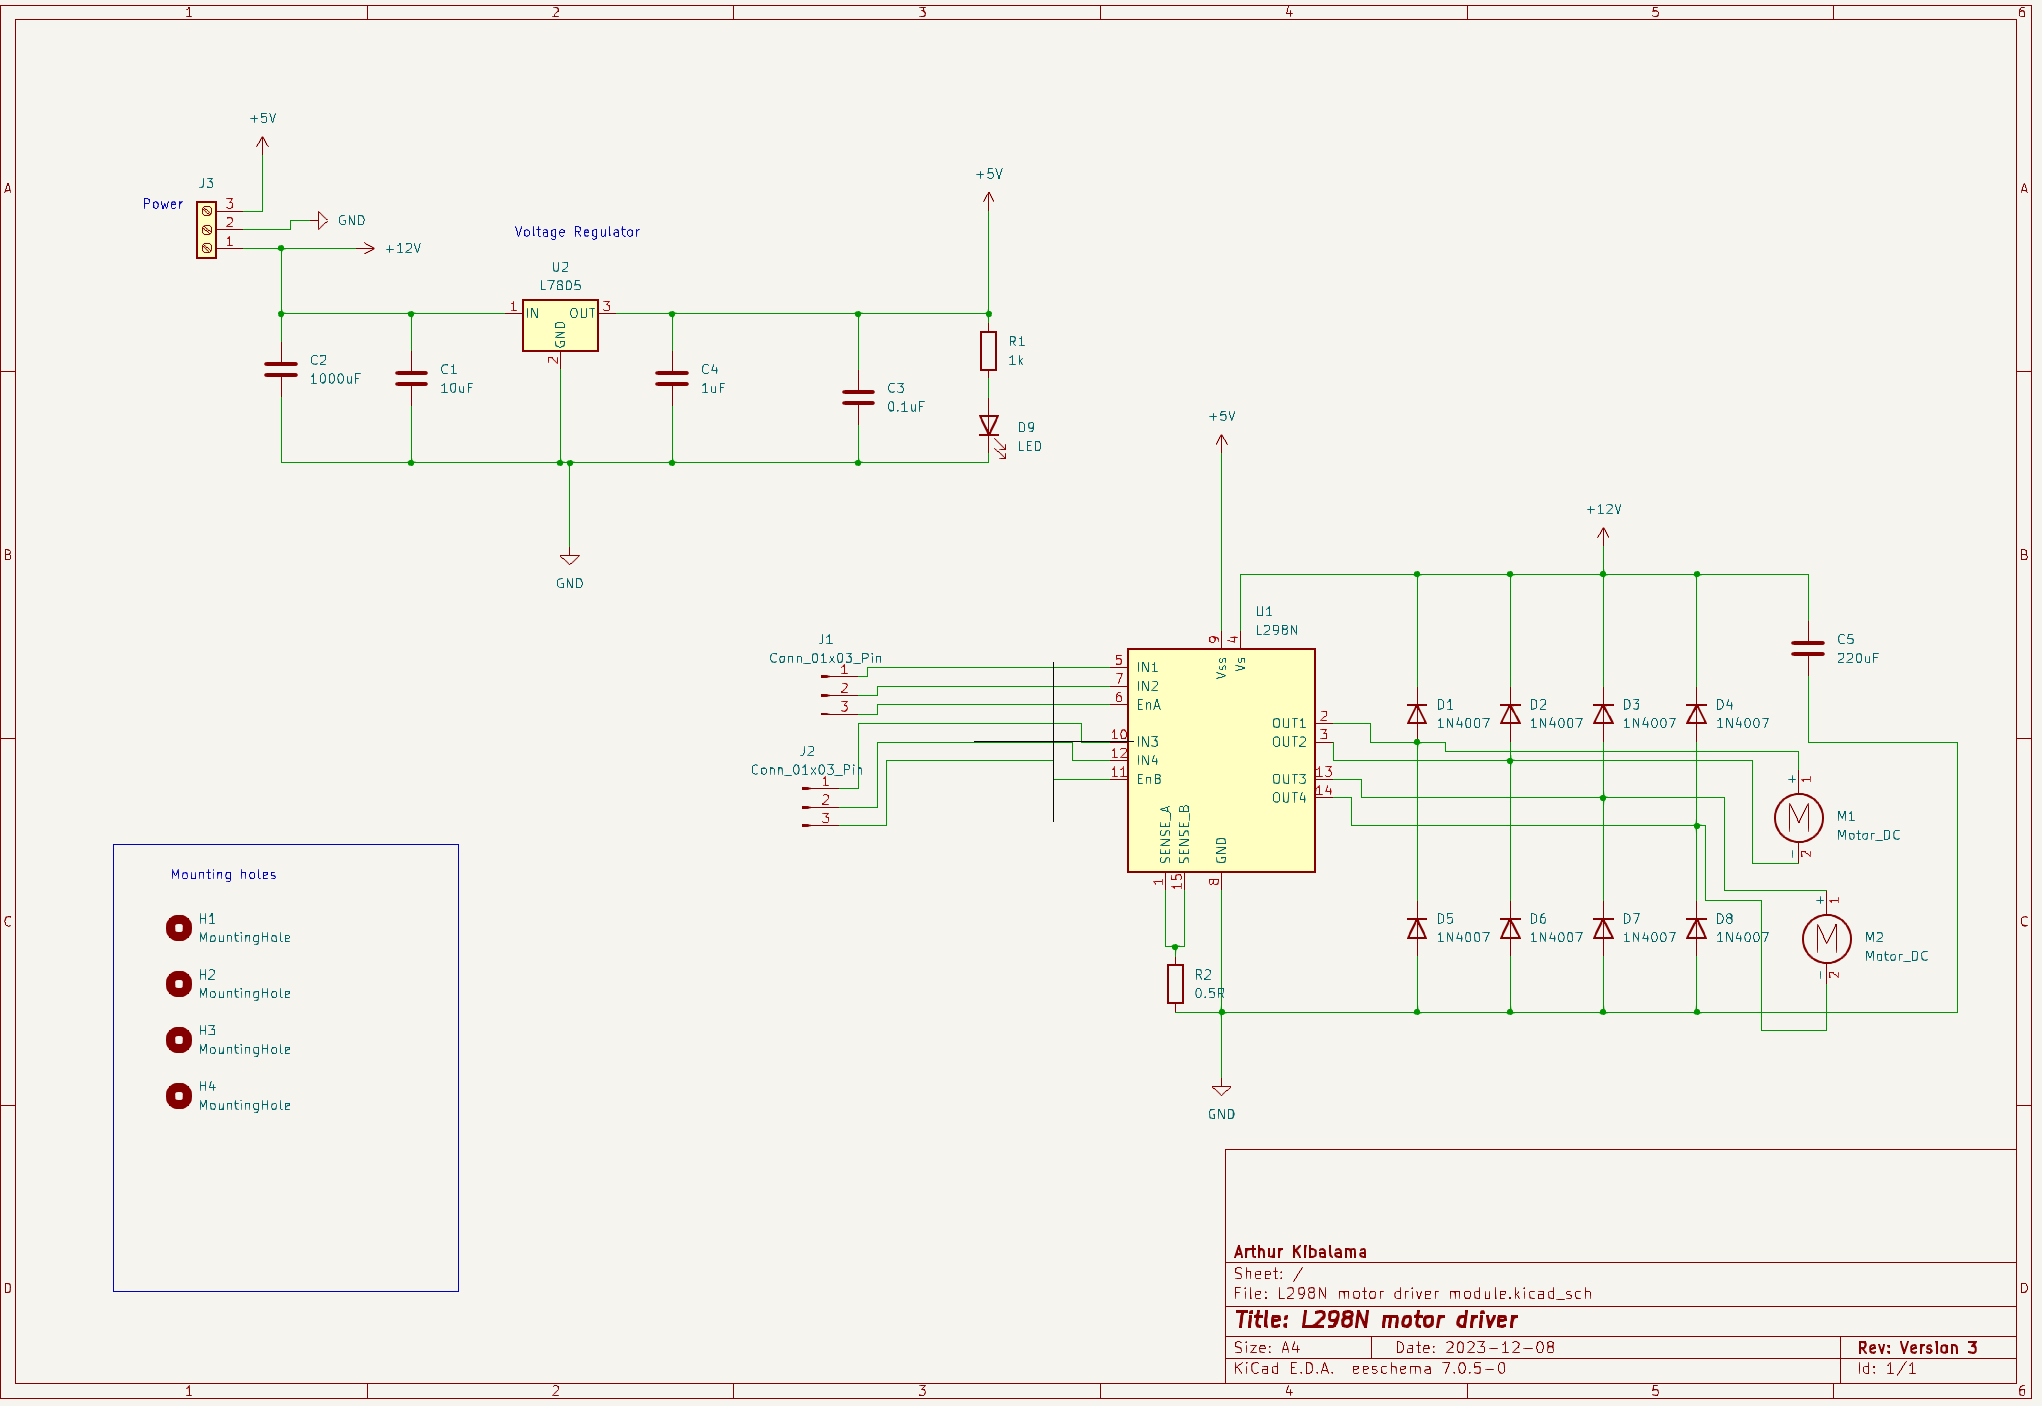
\includegraphics[width=\linewidth]{Screenshot 2023-12-14 at 16.50.36.png}
      \caption{L298n Motordriver Schematic}
    \end{subfigure}
  \end{figure}

  \subsubsection{Tips for creating an optimal Motordriver circuit}
  The L298N is a popular chip used for controlling motors in robots and electronics projects. It can handle two DC motors or one stepper motor and can power them with currents up to 2A each. While it's versatile and can be used in various applications, it's important to design its circuit board layout carefully for it to work well. 
  \begin{itemize}
    \item Power Supply: The L298N requires a dual power supply (Vcc1 and Vcc2) for proper operation. Here I used a voltage regulator, with 6V as output into Vcc2. 
    \item Ground Planes: Proper grounding is critical for the L298N to operate correctly. It is recommended to use a ground plane on the PCB to ensure a low impedance ground path.
    \item Thermal Dissipation: It's crucial to ensure sufficient heat dissipation on the PCB to avert excessive heat buildup. 
    \item Trace Width: The trace width for the power and ground connections should be as wide as possible to minimize resistance and voltage drop.
\end{itemize} 

  \subsubsection{Decoupling Capacitors}
  In the strictest definition, a decoupling capacitor isn't a distinct component per se, instead it characterizes a capacitor's role within an electronic circuit. 
  Its primary function is to enhance stability on the power supply plane by mitigating voltage fluctuations.In any design involving semiconductor ICs, the inclusion of decoupling capacitors is imperative.This is because the voltage supplied to the components deviates significantly from the ideal scenario.Unlike the theoretical perfectly steady line, real-world voltage readings exhibit fluctuations, even with a meticulously clean power supply.The decoupling capacitor operates as a reservoir, contributing to voltage stabilization through two key mechanisms.First, it absorbs excess charges when the voltage surpasses the rated value. Simultaneously, it releases stored charges when the voltage decreases, ensuring a consistently stable power supply.
  Typically, a combination of at least two capacitors with different values is employed to stabilize the voltage supplied to a component's VDD pin. A capacitor around 10 uF serves as a substantial buffer to smooth out low-frequency fluctuations, while a smaller capacitor of approximately 100 nF addresses high-frequency changes in voltage. 

\subsubsection{Waste Management}
Copper recovery from waste printed circuit boards (PCBs) is a topic of interest in the field of waste management. Several studies have been conducted to explore different methods of copper extraction and electrodeposition. These methods include leaching and electrochemical recovery, electrolytic refining, and potential-controlled copper industrial electrolysis. The use of different chemical solutions such as ferric sulphate and cupric chloride has also been investigated. Additionally, mechanical processing and electrometallurgy have been applied for the recovery of copper from PCB scraps. The goal of these studies is to find more efficient and environmentally friendly ways to recover valuable metals from electronic waste.
A study was conducted \cite{copper_recovery}  to optimize the detachment and leaching of metals from waste printed circuit boards (WPCBs). The NaCl-H2SO4-CuSO4 system was used for the leaching process, and Cyclic Voltammetry (CV) was performed to understand the electrochemical behavior of the solution. The results showed that the system was effective in leaching copper from WPCBs, and the presence of other metals did not significantly interfere with the electrochemical recovery of copper. Overall, the study provided insights into the optimization of metal leaching from WPCBs using electrochemical methods. 

\begin{figure}
  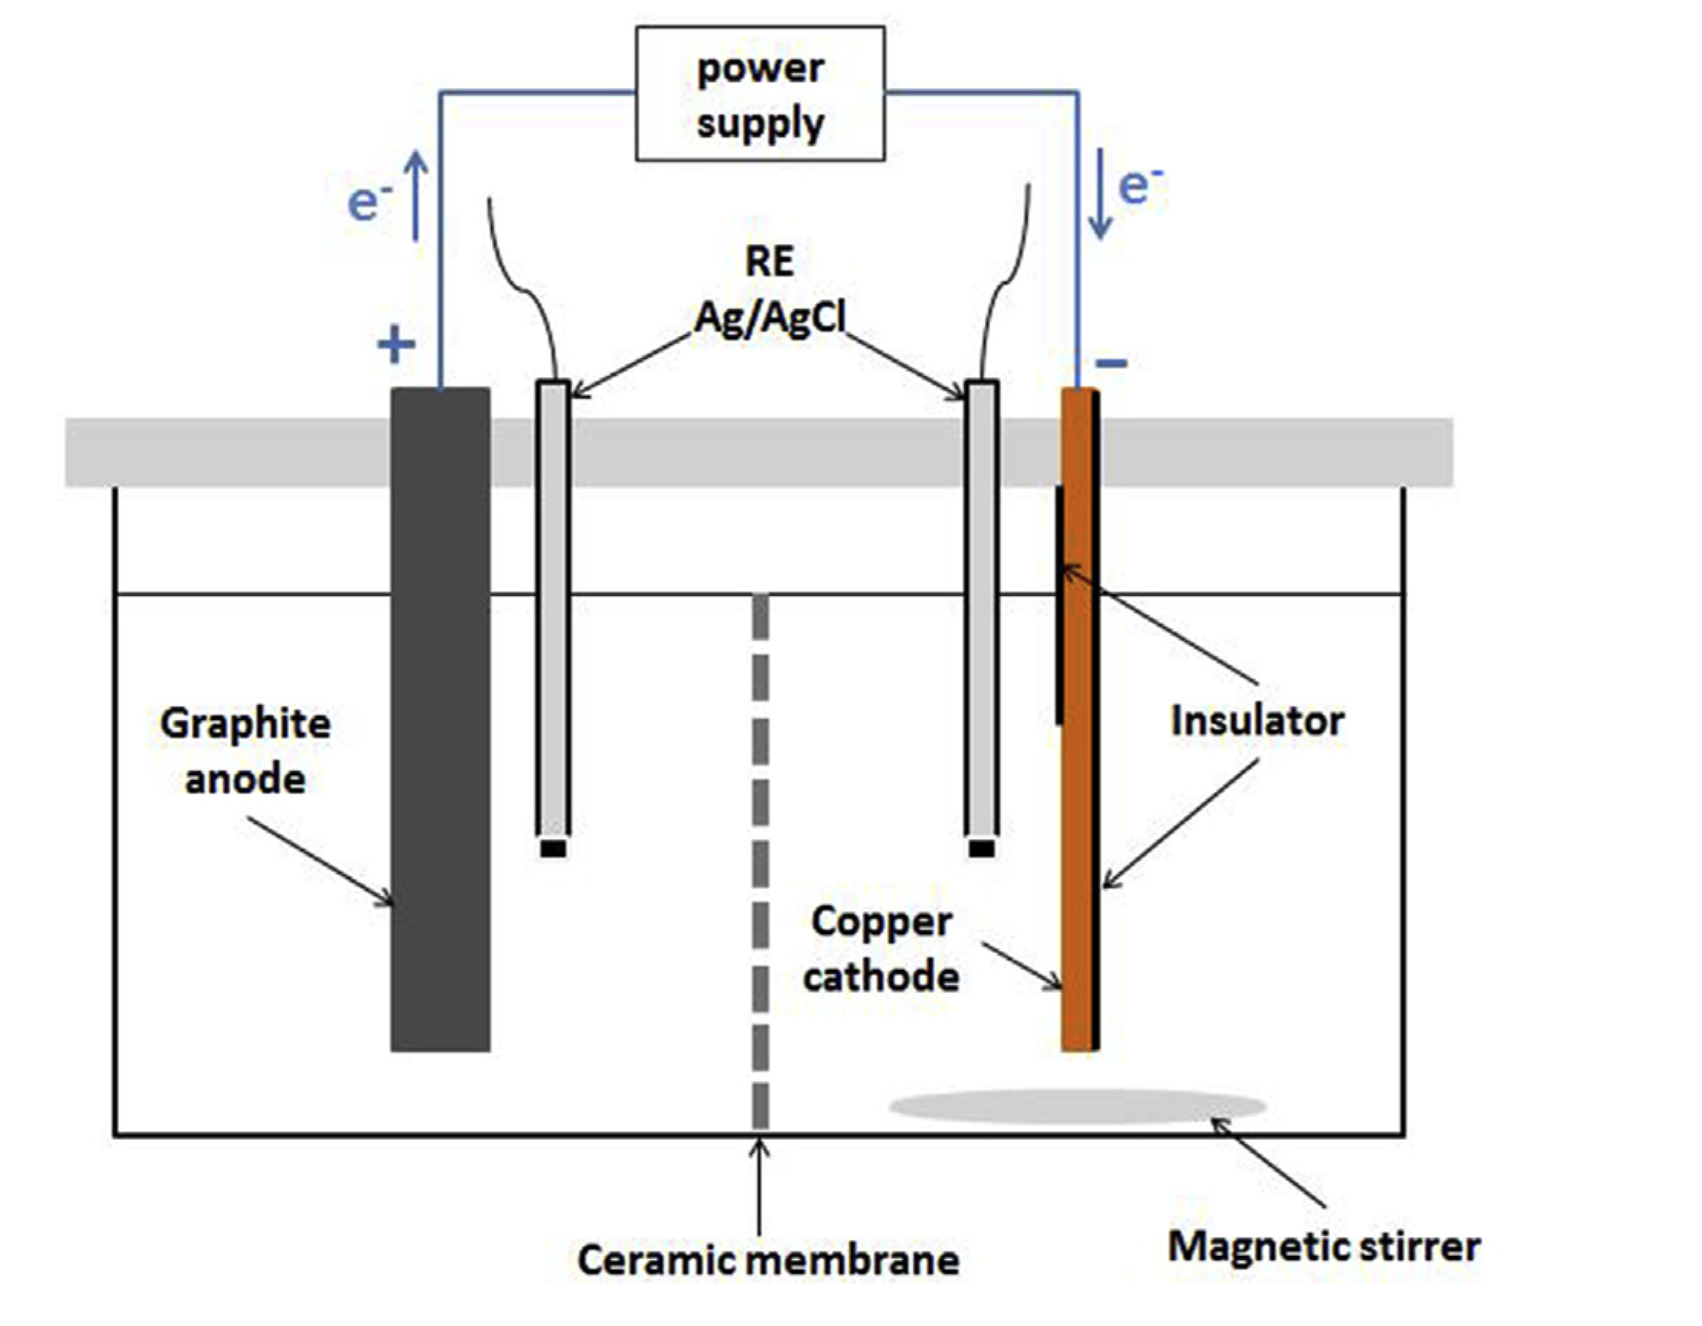
\includegraphics[width=\linewidth]{/Users/arthurkibalama/Documents/GitHub/SDU-SPRO3-LATEX/image/Screenshot 2024-01-01 at 21.09.18.png}
  \caption{Schematic representation of the electrochemical cell used for copper recovery tests.}
  
\end{figure}


\end{document}

